% EGE 2027, task 12. Source IDs and URLs are kept in comments.
% Editable task bank. Append new BankTask blocks at the end of the document.
\documentclass[12pt,a4paper]{article}
\usepackage{physics-textbook}
\usepackage{graphicx,needspace}
\newif\ifShowSolutions
\ifdefined\TutorEdition
  \ShowSolutionstrue
\else
  \ShowSolutionsfalse
\fi
\newcounter{banktask}
\newcommand{\BankTask}[3]{%
  \refstepcounter{banktask}%
  \Needspace{35mm}\par\medskip\noindent\begin{minipage}{\linewidth}%
  \noindent\textbf{\thebanktask.}\quad #2\par
  \ifShowSolutions
    #3\par
    \ifdefined\TutorEdition
      \ifcsname TutorSource#1\endcsname
        \smallskip{\small\csname TutorSource#1\endcsname\par}%
      \fi
    \fi
  \fi
  \end{minipage}\par\medskip
}
\begin{document}


% Source B65453: https://ege.fipi.ru/bank/questions.php?search=1&proj=BA1F39653304A5B041B656915DC36B38&qid=B65453
\BankTask{B65453}{
По прямолинейному проводнику длиной \(50\,\text{см}\), расположенному в однородном магнитном поле с индукцией \(0{,}5\,\text{Тл}\) перпендикулярно линиям индукции поля, течёт ток \(4\,\text{А}\). Определите силу Ампера, действующую на проводник. (в $\text{Н}$).
}{
\smallskip\noindent\textbf{Решение от GPT}\par
Сила Ампера равна \(F=BIl\sin\alpha\). При \(l=0{,}50\,\text{м}\) и \(\alpha=90^\circ\):
\[
F=0{,}5\cdot4\cdot0{,}50=1\,\text{Н}.
\]
Ответ: \(1\,\text{Н}\).
}

% Source 5ED18A: https://ege.fipi.ru/bank/questions.php?search=1&proj=BA1F39653304A5B041B656915DC36B38&qid=5ED18A
\BankTask{5ED18A}{
Прямолинейный проводник длиной \(0{,}2\,\text{м}\), по которому течёт электрический ток, расположен в однородном магнитном поле с индукцией \(B=0{,}6\,\text{Тл}\) под углом \(30^\circ\) к вектору \(\vec{B}\). Сила, действующая на проводник со стороны магнитного поля, равна \(0{,}12\,\text{Н}\). Какова сила тока в проводнике (в $\text{А}$)?
}{
\smallskip\noindent\textbf{Решение от GPT}\par
Из формулы силы Ампера \(F=BIl\sin\alpha\) получаем
\[
I=\frac{F}{Bl\sin\alpha}=\frac{0{,}12}{0{,}6\cdot0{,}2\cdot\sin30^\circ}=2\,\text{А}.
\]
Ответ: \(2\,\text{А}\).
}

% Source c0DF4F: https://ege.fipi.ru/bank/questions.php?search=1&proj=BA1F39653304A5B041B656915DC36B38&qid=c0DF4F
\BankTask{c0DF4F}{
Две частицы с зарядами \(q_1=2q\) и \(q_2=q\) влетают в однородное магнитное поле перпендикулярно вектору магнитной индукции со скоростями \(\upsilon_1=\upsilon\) и \(\upsilon_2=2\upsilon\) соответственно. Определите отношение \(\frac{F_1}{F_2}\) модулей сил, действующих на частицы со стороны магнитного поля в этот момент времени.
}{
\smallskip\noindent\textbf{Решение от GPT}\par
При движении перпендикулярно полю модуль силы Лоренца равен \(F=|q|\upsilon B\). Поэтому
\[
\frac{F_1}{F_2}=\frac{|2q|\upsilon B}{|q|\cdot2\upsilon B}=1.
\]
Ответ: \(1\).
}

% Source 4603AF: https://ege.fipi.ru/bank/questions.php?search=1&proj=BA1F39653304A5B041B656915DC36B38&qid=4603AF
\BankTask{4603AF}{
Две частицы с отношением зарядов $\frac{q_2}{q_1}=\frac{1}{8}$ движутся в однородных магнитных полях, перпендикулярных их скоростям: первая — в поле с индукцией $B_1$; вторая — в поле с индукцией $B_2$. Найдите отношение радиусов траекторий частиц $\frac{R_2}{R_1}$, если их импульсы одинаковы, а отношение модулей индукции $\frac{B_2}{B_1}=2$.
}{
\smallskip\noindent\textbf{Решение от GPT}\par
Радиус траектории $R=\frac{p}{|q|B}$. При одинаковых импульсах
\[
\frac{R_2}{R_1}=\frac{|q_1|B_1}{|q_2|B_2}=8\cdot\frac{1}{2}=4.
\]
Ответ: $4$.
}

% Source D798EB: https://ege.fipi.ru/bank/questions.php?search=1&proj=BA1F39653304A5B041B656915DC36B38&qid=D798EB
\BankTask{D798EB}{
Две частицы с отношением масс $\frac{m_2}{m_1}=4$ движутся в однородных магнитных полях, перпендикулярных их скоростям: первая — в поле с индукцией $\vec{B}_1$; вторая — в поле с индукцией $\vec{B}_2$. Найдите отношение времён $\frac{T_2}{T_1}$, затраченных частицами на один оборот, если их импульсы одинаковы, а отношение радиусов траекторий $\frac{R_2}{R_1}=\frac{1}{2}$.
}{
\smallskip\noindent\textbf{Решение от GPT}\par
Из $p=mv$ и $T=\frac{2\pi R}{v}$ получаем $T=\frac{2\pi Rm}{p}$. При одинаковых импульсах
\[
\frac{T_2}{T_1}=\frac{R_2}{R_1}\frac{m_2}{m_1}=\frac{1}{2}\cdot4=2.
\]
Ответ: $2$.
}

% Source e4eF4A: https://ege.fipi.ru/bank/questions.php?search=1&proj=BA1F39653304A5B041B656915DC36B38&qid=e4eF4A
\BankTask{e4eF4A}{
За \(\Delta t=2\ \text{мс}\) магнитный поток, пронизывающий площадку, которая ограничена проводящим витком, равномерно возрастает от \(2\) до \(8\ \text{мВб}\). Чему равен модуль ЭДС индукции в витке (в $\text{В}$)?
}{
\smallskip\noindent\textbf{Решение от GPT}\par
По закону Фарадея при равномерном изменении потока
\[
|\mathcal{E}|=\frac{|\Delta\Phi|}{\Delta t}=\frac{(8-2)\cdot10^{-3}}{2\cdot10^{-3}}=3\ \text{В}.
\]
Ответ: \(3\ \text{В}\).
}

% Source F1e9FF: https://ege.fipi.ru/bank/questions.php?search=1&proj=BA1F39653304A5B041B656915DC36B38&qid=F1e9FF
\BankTask{F1e9FF}{
За промежуток времени $\Delta t$ магнитный поток, пронизывающий проволочную рамку, равномерно уменьшается от $28\,\text{мВб}$ до нуля. При этом в рамке генерируется ЭДС, равная $7\,\text{мВ}$. Определите промежуток времени $\Delta t$ (в $\text{с}$).
}{
\smallskip\noindent\textbf{Решение от GPT}\par
По закону Фарадея $|\mathcal{E}|=\dfrac{|\Delta\Phi|}{\Delta t}$. Тогда
\[
\Delta t=\frac{28\cdot10^{-3}}{7\cdot10^{-3}}=4\,\text{с}.
\]
Ответ: $4\,\text{с}$.
}

% Source 9C35AF: https://ege.fipi.ru/bank/questions.php?search=1&proj=BA1F39653304A5B041B656915DC36B38&qid=9C35AF
\BankTask{9C35AF}{
В опыте по наблюдению электромагнитной индукции квадратная рамка из одного витка тонкого провода находится в однородном магнитном поле, перпендикулярном плоскости рамки. Индукция магнитного поля равномерно возрастает от $0$ до максимального значения $B_{\text{макс}}$ за время $T$. При этом в рамке возбуждается ЭДС индукции, равная $6\,\text{мВ}$. Какая ЭДС индукции (в $\text{мВ}$) возникнет в рамке, если $T$ уменьшить в $3$ раза, а $B_{\text{макс}}$ уменьшить в $2$ раза?
}{
\smallskip\noindent\textbf{Решение от GPT}\par
Модуль ЭДС равен $|\mathcal{E}|=S B_{\text{макс}}/T$. Поэтому
\[
|\mathcal{E}'|=\frac{S(B_{\text{макс}}/2)}{T/3}=\frac32|\mathcal{E}|=9\,\text{мВ}.
\]
Ответ: $9\,\text{мВ}$.
}

% Source 9FB8B0: https://ege.fipi.ru/bank/questions.php?search=1&proj=BA1F39653304A5B041B656915DC36B38&qid=9FB8B0
\BankTask{9FB8B0}{
На рисунке показан график зависимости магнитного потока $\Phi$, пронизывающего контур, от времени $t$. Найдите модуль ЭДС индукции (в $\text{В}$) в контуре в промежутке времени от $2$ до $4\,\text{с}$.
\begin{center}
\begin{tikzpicture}[x=0.55cm,y=0.275cm,>=stealth]
\draw[->] (0,-9.2)--(0,11.8);
\draw[->] (0,0)--(11.8,0);
\node[above left] at (0,10.5) {$\Phi,\,\text{Вб}$};
\node[below] at (11.5,-0.5) {$t,\,\text{с}$};
\foreach \x in {2,4,6,8,10}{\draw (\x,-0.55)--(\x,0.55);\node[below] at (\x,-0.55) {$\x$};}
\foreach \y in {-8,-4,4,8}{\draw (-0.22,\y)--(0.22,\y);\node[left] at (-0.3,\y) {$\y$};}




\draw (3.25,4)--(4.85,4);
\draw (6.45,4)--(8.1,4);
\draw (9.75,4)--(10,4);
\draw (0,-8)--(.8,-8);
\draw (2.45,-8)--(4,-8);
\draw (2,-.8)--(2,4);
\draw (4,-8)--(4,-4.9);
\draw (10,.25)--(10,3.3);
\draw[thick] (0,4)--(2,4)--(4,-8)--(6,0)--(10,4);
\end{tikzpicture}
\end{center}
}{
\smallskip\noindent\textbf{Решение от GPT}\par
На участке от $2$ до $4\,\text{с}$ поток равномерно изменяется от $4$ до $-8\,\text{Вб}$. По закону Фарадея
\[
|\mathcal{E}|=\frac{|\Delta\Phi|}{\Delta t}=\frac{|-8-4|}{4-2}=6\,\text{В}.
\]
Ответ: $6\,\text{В}$.
}

% Source 4B574A: https://ege.fipi.ru/bank/questions.php?search=1&proj=BA1F39653304A5B041B656915DC36B38&qid=4B574A
\BankTask{4B574A}{
Прямоугольный контур, образованный двумя рельсами и двумя перемычками, находится в однородном магнитном поле, перпендикулярном плоскости контура (см. рисунок). Правая перемычка скользит по рельсам, сохраняя надёжный контакт с ними. Левая перемычка неподвижна. Известны величины: индукция магнитного поля \(B=0{,}1\,\text{Тл}\); расстояние между рельсами \(l=10\,\text{см}\); скорость движения правой перемычки \(\upsilon=2\,\text{м/с}\); сила индукционного тока в контуре \(i_{\text{инд}}=10\,\text{мА}\). Каково сопротивление левой перемычки \(R\) (в $\text{Ом}$)? Сопротивлением рельсов и правой перемычки пренебречь.
\begin{center}
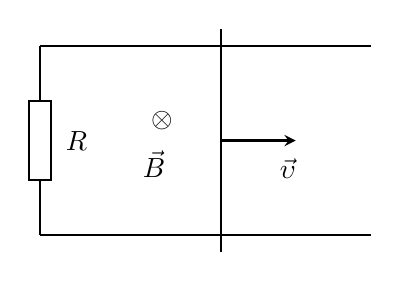
\begin{tikzpicture}[>=stealth, line width=0.8pt]
\draw (0,2.4)--(4.2,2.4);
\draw (0,0)--(4.2,0);
\draw (0,0)--(0,0.7);
\draw (0,1.7)--(0,2.4);
\draw[fill=white] (-0.14,0.7) rectangle (0.14,1.7);
\node[right] at (0.2,1.2) {$R$};
\draw (2.3,-0.22)--(2.3,2.62);
\draw[->] (2.3,1.2)--(3.25,1.2);
\node[below] at (3.15,1.1) {$\vec{\upsilon}$};
\node at (1.55,1.45) {$\otimes$};
\node[below] at (1.45,1.2) {$\vec{B}$};
\end{tikzpicture}
\end{center}
}{
\smallskip\noindent\textbf{Решение от GPT}\par
ЭДС движения равна \(\mathcal{E}=Bl\upsilon\). По закону Ома
\[
R=\frac{Bl\upsilon}{i_{\text{инд}}}=\frac{0{,}1\cdot0{,}10\cdot2}{0{,}010}=2\,\text{Ом}.
\]
Ответ: \(2\,\text{Ом}\).
}

% Source DB72A1: https://ege.fipi.ru/bank/questions.php?search=1&proj=BA1F39653304A5B041B656915DC36B38&qid=DB72A1
\BankTask{DB72A1}{
Сила тока в катушке с индуктивностью \(0{,}2\,\text{Гн}\) за \(0{,}05\,\text{с}\) равномерно увеличилась от \(2\,\text{А}\) до \(5\,\text{А}\). Чему равен модуль ЭДС самоиндукции в катушке (в $\text{В}$)?
}{
\smallskip\noindent\textbf{Решение от GPT}\par
\[
|\mathcal{E}_{\text{си}}|=L\frac{|\Delta I|}{\Delta t}=0{,}2\cdot\frac{5-2}{0{,}05}=12\,\text{В}.
\]
Ответ: \(12\,\text{В}\).
}

% Source B8FD36: https://ege.fipi.ru/bank/questions.php?search=1&proj=BA1F39653304A5B041B656915DC36B38&qid=B8FD36
\BankTask{B8FD36}{
При равномерном изменении силы тока в катушке на \(10\,\text{А}\) за \(0{,}02\,\text{с}\) в ней возникает ЭДС самоиндукции, равная \(200\,\text{В}\). Чему равна индуктивность катушки (в $\text{Гн}$)?
}{
\smallskip\noindent\textbf{Решение от GPT}\par
Из \(|\mathcal{E}_{\text{си}}|=L|\Delta I|/\Delta t\) получаем
\[
L=\frac{|\mathcal{E}_{\text{си}}|\Delta t}{|\Delta I|}=\frac{200\cdot0{,}02}{10}=0{,}4\,\text{Гн}.
\]
Ответ: \(0{,}4\,\text{Гн}\).
}

% Source 159D34: https://ege.fipi.ru/bank/questions.php?search=1&proj=BA1F39653304A5B041B656915DC36B38&qid=159D34
\BankTask{159D34}{
В катушке индуктивностью \(1\,\text{мГн}\) сила тока в течение \(0{,}1\,\text{с}\) равномерно возрастает от \(0\) до некоторого конечного значения. При этом в катушке наблюдается ЭДС самоиндукции, модуль которой равен \(0{,}2\,\text{В}\). Определите конечное значение силы тока в катушке (в $\text{А}$).
}{
\smallskip\noindent\textbf{Решение от GPT}\par
По закону самоиндукции \(|\mathcal{E}|=L\dfrac{\Delta I}{\Delta t}\). Начальный ток равен нулю, поэтому
\[
I=\frac{|\mathcal{E}|\Delta t}{L}=\frac{0{,}2\cdot0{,}1}{10^{-3}}=20\,\text{А}.
\]
Ответ: \(20\).
}

% Source 31DAF4: https://ege.fipi.ru/bank/questions.php?search=1&proj=BA1F39653304A5B041B656915DC36B38&qid=31DAF4
\BankTask{31DAF4}{
На рисунке приведён график зависимости силы тока от времени в электрической цепи, содержащей катушку, индуктивность которой равна \(1\,\text{мГн}\). Определите модуль ЭДС самоиндукции (в $\text{мкВ}$) в интервале от \(0\) до \(5\,\text{с}\).
\begin{center}
\begin{tikzpicture}[x=0.25cm,y=0.142cm,>=stealth]
\draw[thin] (0,10)--(20,10) (0,20)--(20,20) (0,30)--(20,30);
\draw[thin] (5,0)--(5,30) (10,0)--(10,30) (15,0)--(15,30) (20,0)--(20,30);
\draw[->] (0,0)--(23,0) node[right] {\(t,\,\text{с}\)};
\draw[->] (0,0)--(0,39);
\node[anchor=east] at (-0.8,38) {\(I,\,\text{мА}\)};
\node[below left] at (0,0) {\(0\)};
\foreach \x in {5,10,15,20} \node[below] at (\x,0) {\(\x\)};
\foreach \y in {10,20,30} \node[left] at (0,\y) {\(\y\)};
\draw[thick] (0,0)--(5,30)--(10,20)--(15,20)--(20,0);
\end{tikzpicture}
\end{center}
}{
\smallskip\noindent\textbf{Решение от GPT}\par
В интервале от \(0\) до \(5\,\text{с}\) ток равномерно возрастает от \(0\) до \(30\,\text{мА}\). Тогда
\[
|\mathcal{E}|=L\frac{|\Delta I|}{\Delta t}=10^{-3}\frac{30\cdot10^{-3}}{5}=6\cdot10^{-6}\,\text{В}=6\,\text{мкВ}.
\]
Ответ: \(6\).
}

% Source 458c72: https://ege.fipi.ru/bank/questions.php?search=1&proj=BA1F39653304A5B041B656915DC36B38&qid=458c72
\BankTask{458c72}{
Чему равна индуктивность катушки (в $\text{мГн}$), если при силе тока \(5\,\text{А}\) энергия её магнитного поля равна \(12{,}5\,\text{мДж}\)?
}{
\smallskip\noindent\textbf{Решение от GPT}\par
Энергия магнитного поля катушки \(W=\dfrac{LI^2}{2}\), поэтому
\[
L=\frac{2W}{I^2}=\frac{2\cdot12{,}5\cdot10^{-3}}{5^2}=10^{-3}\,\text{Гн}=1\,\text{мГн}.
\]
Ответ: \(1\).
}

% Source D747BC: https://ege.fipi.ru/bank/questions.php?search=1&proj=BA1F39653304A5B041B656915DC36B38&qid=D747BC
\BankTask{D747BC}{
Какова энергия магнитного поля катушки индуктивностью \(0{,}4\,\text{Гн}\), если сила тока в катушке равна \(6\,\text{А}\) (в $\text{Дж}$)?
}{
\smallskip\noindent\textbf{Решение от GPT}\par
Энергия магнитного поля катушки:
\[
W=\frac{LI^2}{2}=\frac{0{,}4\cdot 6^2}{2}=7{,}2\,\text{Дж}.
\]
Ответ: \(7{,}2\,\text{Дж}\).
}

% Source C453EB: https://ege.fipi.ru/bank/questions.php?search=1&proj=BA1F39653304A5B041B656915DC36B38&qid=C453EB
\BankTask{C453EB}{
Энергия магнитного поля катушки с током равна \(0{,}64\,\text{Дж}\). Индуктивность катушки равна \(20\,\text{мГн}\). Какова сила тока в катушке (в $\text{А}$)?
}{
\smallskip\noindent\textbf{Решение от GPT}\par
Из \(W=LI^2/2\), учитывая \(L=20\,\text{мГн}=0{,}020\,\text{Гн}\), получаем:
\[
I=\sqrt{\frac{2W}{L}}=\sqrt{\frac{2\cdot0{,}64}{0{,}020}}=8\,\text{А}.
\]
Ответ: \(8\,\text{А}\).
}

% Source 7FABFc: https://ege.fipi.ru/bank/questions.php?search=1&proj=BA1F39653304A5B041B656915DC36B38&qid=7FABFc
\BankTask{7FABFc}{
За время $\Delta t=2\,\text{с}$ магнитный поток через площадку, ограниченную проволочной рамкой, равномерно уменьшается от некоторого значения $\Phi$ до нуля. При этом в рамке генерируется ЭДС индукции, равная $10\,\text{мВ}$. Определите начальный магнитный поток $\Phi$ через рамку. (в $\text{мВб}$).
}{
\smallskip\noindent\textbf{Решение от GPT}\par
По закону Фарадея $|\mathcal E|=|\Delta\Phi|/\Delta t=\Phi/\Delta t$. Поэтому $\Phi=|\mathcal E|\Delta t=10\cdot10^{-3}\cdot2=0{,}020\,\text{Вб}=20\,\text{мВб}$. Ответ: $20\,\text{мВб}$.
}

% Source 91A4F6: https://ege.fipi.ru/bank/questions.php?search=1&proj=BA1F39653304A5B041B656915DC36B38&qid=91A4F6
\BankTask{91A4F6}{
Прямолинейный проводник длиной $L$, по которому протекает ток $I$, помещён в однородное магнитное поле перпендикулярно линиям индукции $\vec B$. Во сколько раз уменьшится сила Ампера, действующая на проводник, если его длину увеличить в $3$ раза, индукцию магнитного поля уменьшить в $6$ раз, а силу тока в проводнике поддерживать прежней?
}{
\smallskip\noindent\textbf{Решение от GPT}\par
$F=BIL$, поэтому $F_2/F_1=(B_2/B_1)(L_2/L_1)=\frac16\cdot3=\frac12$. Ответ: в $2$ раза.
}

% Source D0F00F: https://ege.fipi.ru/bank/questions.php?search=1&proj=BA1F39653304A5B041B656915DC36B38&qid=D0F00F
\BankTask{D0F00F}{
Два прямолинейных проводника помещены в однородное магнитное поле перпендикулярно линиям индукции магнитного поля $\vec B$. Длина первого проводника равна $L$, сила протекающего по нему тока равна $I$. Длина второго проводника равна $0{,}8L$, сила протекающего по нему тока равна $0{,}5I$. Чему равно отношение $F_2/F_1$ модулей сил Ампера, действующих на проводники?
}{
\smallskip\noindent\textbf{Решение от GPT}\par
$F=BIL$, поэтому $F_2/F_1=(I_2/I_1)(L_2/L_1)=0{,}5\cdot0{,}8=0{,}4$. Ответ: $0{,}4$.
}

\end{document}
